\documentclass{LULCSProject}
\usepackage{amsmath}
\usepackage{enumitem}
\usepackage{listings, listings-rust}
\usepackage{graphicx}
\usepackage{todonotes}
\newcommand{\tvect}[3] { \ensuremath{\Bigl(\negthinspace\begin{smallmatrix}#1\\#2\\#3\end{smallmatrix}\Bigr)}}
\newcommand{\twovect}[2] { \ensuremath{\left(\negthinspace\begin{smallmatrix}#1\\#2\end{smallmatrix}\right)}}


\title{An Open Source Smart home Platform}
\author{Niklas Harnish}
\date{12/05/2023}
%\BSc % \MEng \BEng etc. 
\supervisor{Dr Amna Asif}

\wordcount{0} % number of words in your report 


\abstract{Put your abstract here. You should create a short abstract (200
words at maximum) which is on a page by itself. The abstract should be
a very high-level overview: for example 1--2 sentences on the aims of
the project, 1--2 sentences on the kind of design, implementation, or
empirical work undertaken, and 2--3 sentences summarising the primary
contribution or findings from your work. The abstract appears in the
front matter of the report: after your title page but before the table
of contents.

what should go in here:
\list{}
    \item aims
    \item design
    \item implementation
    \item findings and primary contribution

}


\declaration{
  Put some text similar to the following in here:\\[.5em]
I certify that the material contained in this dissertation is my own work and does not contain
unreferenced or unacknowledged material. I also warrant that the above statement applies to the
implementation of the project and all associated documentation. Regarding the electronically
submitted work, I consent to this being stored electronically and copied for assessment purposes,
including the School's use of plagiarism detection systems in order to check the integrity of
assessed work.\\
I agree to my dissertation being placed in the public domain, with my name explicitly included
as the author of the work.\\
Name:\\
Date:
}

\dedication{
  If you want to dedicate to someone in particular
}

\acknowledgements{
  General acknowledgements \ldots

  your supervisor, your family, your
  friends, \ldots
}

\begin{document}

\maketitle

\pagenumbering{Roman}

%\tableofcontents

\listoffigures
\newpage
% \begingroup
% \let\clearpage\relax
\listoftables
%\endgroup

\newpage
\pagenumbering{arabic}

%%
%% include your chapters here
%%
\chapter{Introduction} \label{cha:intro}
\todo{actually write this section}Will write a couple of words about the project 
here, similar projects, inspirations etc. Citation here to remember how to do it 
:)

\section{Aims \& Objectives} \label{sec:intro:aims}
When researching available smart home technology, one major gap I came across 
was the availability of open source software. While options exist for someone 
interested in connecting their proprietary device to an open source platform 
(view \todo{find the link to this}), there was no solution for anyone looking to 
build their own device and then connect it to an open source hub. In fulfilling 
this goal, to build an open source platform for both devices and the hub they 
will connect to, there are multiple objectives that will need to be met along 
the way:
\begin{enumerate}
    \item Create a Library and API (Application Programming Interface) for 
        building smart home devices.
    \item Build a Server with an API for the smart home devices to communicate 
        with. This will act as a hub and will control clients connected to it.
         \begin{enumerate}
             \item This API should be well documented, so a user can interact 
                 with the hub, without using the Library.
         \end{enumerate}
     \item Create a frontend, which will be populated with devices currently 
         connected to the smart home. It will also be used to control clients 
         connected to the server.
         \begin{enumerate}
             \item The API provided by the server for this frontend should also 
                 be easy to use, so the user can create their own frontend 
                 environment.
         \end{enumerate}
     \item The code of all of the above should be hosted in a public repository, 
         with instructions for how to build and use every component of the 
         system.
         \begin{enumerate}
             \item An appropriate license should also be selected for this 
                 repository, so the code within it can be copied or modified by 
                 third parties.
             \item This repository should provide important links and provide 
                 information on the inner workings of the system, to support 
                 interested parties.
         \end{enumerate}
\end{enumerate}
    
\section{Project Overview} \label{sec:intro:overview} \todo{ask about this 
section}
\textit{Each bullet point below would give a small summary of the section}
\begin{enumerate}
    \item \textbf{Background Research} 
    \item \textbf{Design of the System \& Technology Decisions}
    \item \textbf{Implementation}
    \item \textbf{Results}
    \item \textbf{Conclusion and Reflection}
chapter1.tex
\end{enumerate}


% Always start your chapter on a new page!
\newpage
\chapter{Background} \label{cha:chapter2}

\section{IoT System Architectures} \label{sec:chap2:architectures}
Kamienski et al. describe a simple three layer architecture of an IoT system in \cite{DesigningOpenIotSystem}. Within this architecture, the top layer is the "Input System", from which any data that will influence the decisions of the IoT system will come from. Included in this are sensors, but also user facing interfaces. The second layer, known as the "Process System", is where any algorithms are run and system behavioral decisions are made. The goal of this layer is to gain an "improved understanding of the system where the  data comes from" \cite{DesigningOpenIotSystem}. The bottom layer is the "Output System", which are where decisions made by the Process System will be enacted. This is often represented as the devices connected to the IoT system.

This three layer architecture is expanded upon by Bansal and Kumar within \cite{IotEcosystemSurvey}, where three more architectures are described which expand upon the ideas within the three layer architecture. They are however more specialized than the three layer architecture. The first of these is a "Middleware Based" architecture, which can take many forms, but is usually combined with another type of architecture, with a middleware layer. The different types are described in detail by Zhang et al. in \cite{MiddlewareIOTSurvey}. The second is known as a "Fog Based" architecture, where certain tasks, usually those with less processing requirements, are calculated on device to reduce latency. More computationally expensive tasks are however calculated on a server in the cloud \cite{IoTArchitectures}.

The most relevant architecture to this report is known as a "Service Based" architecture (SBA). The SBA is defined around the concept of the Service Oriented Architectural (SOA) style \cite{InteractingSoaBasedIot} of software design. SOA is defined by the Open Group Foundation as an "architectural style that supports service-orientation", where a service is a "logical representation of a repeatable business activity that has a specified outcome" \cite{SoaSourceBook}. Each service is a "black box" any device interacting with it. Other devices use interfaces and API endpoints to make requests to the service and receive a result. A SOA is comprised of many different services. In SBA, services are used to offer device functionality using interfaces, often using web based concepts such as SOAP or REST APIs \cite{TrustManagementSoaIot}. This allows devices with different capabilities and purposes to interact with the same system, allowing for an IoT system that is more flexible. 


\section{The Smart Home System} \label{sec:chap2:smarthome}
Sethi and Sarangi define six components that need to be present within a social IoT setting. A social IoT system is defined as a IoT system where devices form relationships with other devices. While our smart home system will not be a social IoT system, some of these concepts are still of interest. These are: \todo{ask if this is ok with citation as its quite similar}
\begin{enumerate}
    \item ID: the device within the system needs to have a way of identifying 
        it.
    \item Meta-data: the device should have information regarding its form and 
        purpose
    \item Security Controls: the system should have some way of distinguishing 
        between different users. It should also be able to distinguish what 
        types of devices it can connect to or can connect to it.
    \item Service Discovery: each device should be able to discover other 
        devices connected to the system and what services they offer.
\end{enumerate}

There are some specific constraints specific to Smart Homes. Reliability is a key concern, due to the lack of a trained professional being available to fix any issues that arise. This is contrast to more industrial IoT settings, where there might be someone to fix any issues that arise. Another concern is the security and privacy of the system. Due to smart homes inherently having access to sensitive data (due to their position in someone's home), one must ensure that the system is both ethically sound and secure. The issue of security is further discussed in Subsection~\ref{sec:chap2:security}.
\todo{further add to this section, just not sure what yet}

\section{APIs and Web Interfaces} \label{sec:chap2:frontend}
\section{Security} \label{sec:chap2:security}
\section{Networking} \label{sec:chap2:networking}
\section{Open Source and Licensing} \label{sec:chap2:opensource}



%%
%% You bib file
%%
\newpage
\bibliography{report}

\newpage
\appendix
%%
%% Your appendices
%%
\chapter{Original Project Proposal}
\label{chap:A1}

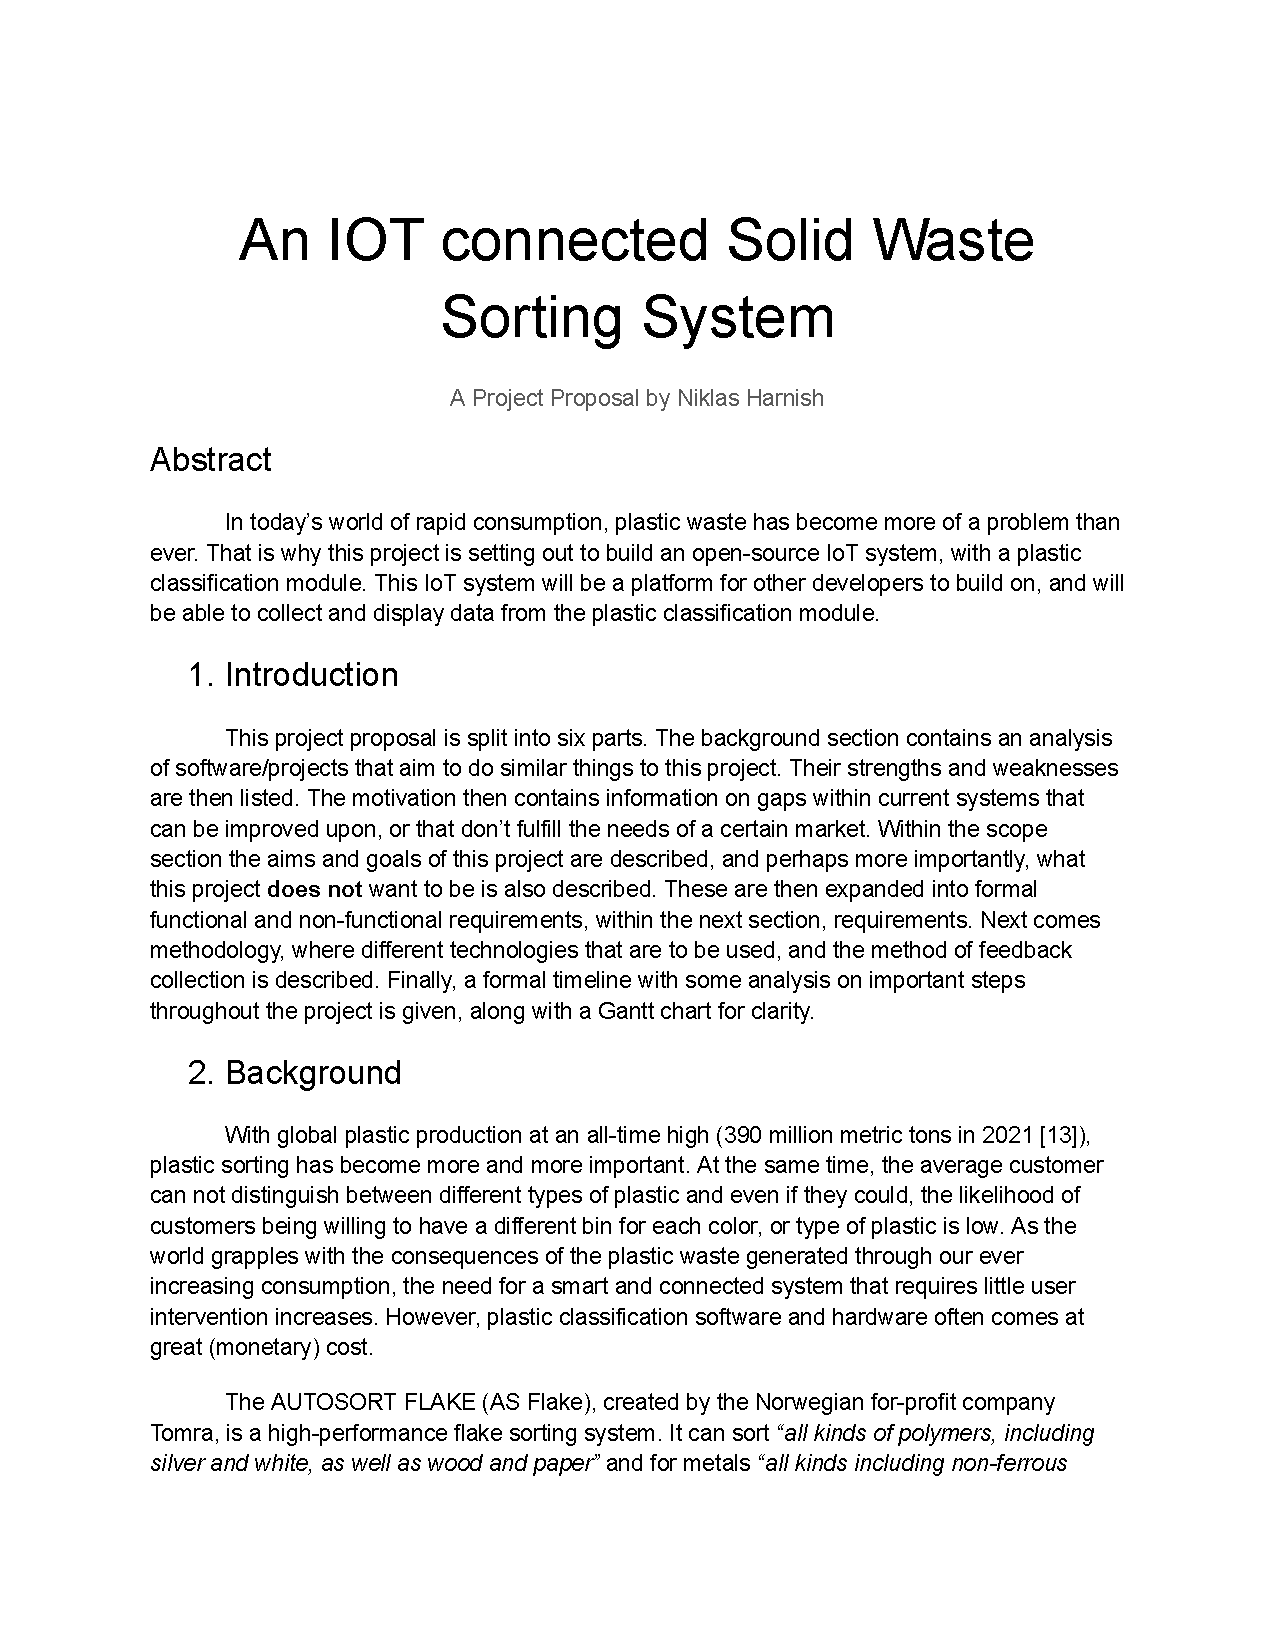
\includepdf[pages=-]{project_proposal.pdf}

\newpage

\chapter{Another Appendix Chapter}
\label{chap:A2}

This could be about your experiments

\end{document}
